\section{Introduction}
In-memory collections of data often need efficient processing. For on-disk
data, efficient processing is already provided by database management systems~(DBMS) thanks to
their query optimizers, which support many optimizations specific to the domain
of collections. Moving in-memory data to DBMSs, however,
typically does not improve performance~\citep{Stonebraker07}, and query optimizers cannot
be reused separately since DBMS are typically monolithic and their optimizers deeply integrated.
A few collection-specific optimizations, such as shortcut
fusion~\citep{Gill93shortcut}, are supported by compilers for purely
functional languages such as Haskell. However, the implementation techniques for
those optimizations do not
generalize to many other ones, such as support for indexes. In
general, collection-specific optimizations are not supported by the general-purpose
optimizers used by typical (JIT) compilers.

%Therefore, programs often manipulate collections using languages where automatic
%domain-specific optimizations are not supported, and thus perform some
%collection-related optimizations by hand.%~\citep{AOP}.

% High-level is missing. Maybe put that in the conclusion.
%Programmers would benefit from domain-specific
%optimizations which are not supported by 
%current general-purpose optimizers.
%Such optimizations are supported instead by query optimizers in database
%management systems (DBMS). However, such query optimizers cannot be used on their own because
%database systems are usually monolithic; moving collection processing to a
%DBMS, instead, is not always appropriate nor easy since they are geared toward on-disk data and support a
%quite different data model: in-memory data is typically represented as an object
%graph, which is not easy to convert to flat relational data; specialized toolkit
%exist, but require a high amount of control from the programmer~\citep{Meijer11CoSQL}.
%%it is not trivial to convert in-memory data (object
%%graphs) to flat relational data, that is, to perform object-relational
%%mapping~\citep{Meijer11CoSQL}.
%A similar mismatch exists between SQL and most
%general-purpose programming languages: expressing general-purpose
%computations in SQL is therefore often problematic~\citep{Stonebraker07,Yu08}.
Therefore programmers, when needing
collection-related optimizations, perform them manually. To allow that, they are often forced to perform manual
inlining~\citep{Peyton-Jones02}.
But manual inlining
modifies source code by combining distinct functions together, while often distinct
functions should remain distinct, because they deal with different concerns, or
because one function need to be reused in a different context.
In either case, manual inlining reduces modularity --- defined here as the
ability to abstract behavior in a separate function (possibly part of a
different module) to enable reuse and improve understandability.%
%In general, to preserve modularity.
%When a function is separated because it is part of another module, manual
%inlining will reduce modularity.

%can reduce modularity.% and in particular violates \emph{information hiding}.
%Programs are partitioned in different modules, that is modularized, for many
%reasons, for instance to separate different implementation concerns and hide
%implementation details from one another. The smallest modularization
%Inlining combines together code from different functions
%Code fragments are divided in differen modules to hide implementation details between
%abstraction barriers.
%Manual inlining modifies source code by combining functions, even if it would
%be better to keep them distinct, because for instance they are part of different
%modules, or they have logically different goals.
%---we assume for some good reason, for instance because they are part of different modules.
%When two functions are logically distinct, 

For these reasons, currently developers need to choose between modularity and
performance, as also highlighted by
\citet{AOP} on a similar example.
Instead, we envision that they should rely on an automatic optimizer performing inlining
and collection-specific optimizations. They would then achieve both performance and modularity.%
\footnote{In the terminology of \citet{AOP}, our goal is to be able to decompose
different \emph{generalized procedures} of a program according to its primary
decomposition, while separating the handling of some performance concerns. To
this end, we are modularizing these performance concerns into a
metaprogramming-based optimization module, which we believe
could be called, in that terminology, \emph{aspect}.}

One way to implement such an optimizer would be to extend the compiler of the language with a collection-specific optimizer, or 
to add some kind of external preprocessor to the language. However, such solutions would be rather brittle (for instance, they lack
composability with other language extensions) and they would preclude optimization opportunities that arise only at runtime.

For this reason, our approach is implemented as an embedded domain-specific language, that is, as a regular library.
We call this library \LoSDef. \LoS\ consists of a domain-specific language (DSL) for queries on collections based on the Scala collections API\@. 
This DSL is implemented as an embedded DSL (EDSL) for Scala. An expression in this EDSL produces at run time an \emph{expression tree} in the host language: a data structure which represents the query to execute, similar to an abstract syntax tree (AST) or a query plan. Thanks to the extensibility of Scala, expressions in this language look almost identical to expressions with the same meaning in Scala.
When executing the query, \LoS\ optimizes and compiles these expression trees for more efficient execution. Doing optimization at run time, instead of compile-time, avoids the need for control-flow analyses to determine which code will be actually executed~\citep{Chambers10}, as we will see later.

We have choosen Scala \citep{Odersky11book} to implement our library for two reasons: (i) Scala is a good meta-language for embedded DSLs, because it is syntactically
flexible and has a powerful type system, and (ii) Scala has a sophisticated collections library with an attractive syntax (for-comprehensions) to specify queries.

To evaluate \LoS, we study queries of the FindBugs tool~\citep{DBLP:journals/sigplan/HovemeyerP04}.
We rewrote a set of queries to use the Scala collections API and show that  modularization incurs significant performance overhead. Subsequently, we consider versions of the same queries using \LoS{}. 
We demonstrate that the automatic optimization can reconcile modularity and performance in many cases. Adding advanced optimizations such as indexing can even improve the performance of the analyses beyond the original non-modular analyses.
 
Overall, our main contributions are the following:
\begin{itemize}
\item We illustrate the tradeoff between modularity and performance when manipulating collections, caused by the lack of domain-specific optimizations~(Sec.~\ref{sec:motivation}). Conversely, we illustrate how domain-specific optimizations lead to more readable and more modular code (Sec.~\ref{sec:solution}).
\item We present the design and implementation of \LoS, an embedded DSL for queries on collections in Scala (Sec.~\ref{sec:implementation}).
%\LoS\ makes heavy usage of advanced Scala features to preserve the ``look and feel'' of native Scala queries
% and is hence a significant showcase for these features~(Sec.~\ref{sec:implementation}).
 \item We evaluate \LoS\ to show that it supports writing queries that are at the same time modular and fast. We do so by re-implementing several code analyses of the FindBugs tool.
 The resulting code is more modular and/or more efficient, in some cases by orders of magnitude.
 In these case studies, we measured average speedups of \avgSpeedupT{} with a maximum of \maxSpeedupT{}~(Sec.~\ref{sec:evaluation}).
\end{itemize}

\section{Motivation}
\label{sec:motivation}

In this section, we show how the absense of collection-specific optimizations
forces programmers to trade modularity against performance, which motivates our design of {\LoS} to resolve this conflict.

As our running example through the paper, we consider representing and querying a simple in-memory bibliography. A book has, in our schema, a title, a publisher and a list of authors. Each author, in turn, has a first and last name. We represent authors and books as instances of the Scala classes \code{Author} and \code{Book} shown in Fig.~\ref{fig:schema}. The class declarations list the type of each field: Titles, publishers, and first and last names are all stored in fields of type \code{String}. The list of authors is stored in a field of type \code{Seq[Author]}, that is, a sequence of authors -- something that would be more complex to model in a relational database.
The code fragment also defines a collection of books named \code{books}.
\begin{figure}[t]
\centering
\begin{lstlisting}
package schema
case class Author(firstName: String, lastName: String)
case class Book(title: String, publisher: String,
  authors: Seq[Author])

val books: Set[Book] = Set(
  new Book("Compilers: Principles, Techniques and Tools",
       "Pearson Education",
       Seq(new Author("Alfred V.", "Aho"),
           new Author("Monica S.", "Lam"),
           new Author("Ravi", "Sethi"),
           new Author("Jeffrey D.", "Ullman"))
  /* other books ... */)
\end{lstlisting}
\caption{Definition of the schema and of some content.}
\label{fig:schema}
\end{figure}

As a common idiom to query such collections, Scala provides \emph{for-comprehensions}.
For instance, the for\-/comprehension computing \code{records} in Fig.~\ref{fig:query} finds all books published by Pearson Education and yields, for each of those books, and for each of its authors, a record containing the book title, the full name of that author and the number of additional coauthors.
The \emph{generator} \code{book <- books} functions like a loop header: The remainder of the for-comprehension is executed once per book in the collection. Consequently, the \emph{generator} \code{author <- book.authors} starts a nested loop.
The return value of the for-comprehension is a collection of all yielded
records. Note that if a book has multiple authors, this for-comprehensions will
return multiple records relative to this book, one for each author.

\begin{figure}[t]
\centering
\begin{lstlisting}
case class BookData(title: String, authorName: String,
  coauthors: Int)

val records =
  for {
    book <- books
    if book.publisher == "Pearson Education"
    author <- book.authors
  } yield new BookData(book.title,
                 author.firstName + " " +
                 author.lastName,
                 book.authors.size - 1)

def titleFilter(records: Set[BookData],
    keyword: String) =
  for {
    record <- records
    if record.title.contains(keyword)
  } yield (record.title, record.authorName)

val res = titleFilter(records, "Principles")
\end{lstlisting}
\caption{Our example query on the schema in Fig.~\ref{fig:schema}, and a function which postprocesses its result.}
\label{fig:query}
\end{figure}

We can further process this collection with another for-comprehension, possibly
in a different module. For example, still in Fig.~\ref{fig:query}, the function
\code{titleFilter} filters book titles containing the word "Principles", and
drops from each record the number of additional coauthors.

In Scala, the implementation of for-comprehensions is not fixed. Instead, the
compiler desugars a for-comprehension to a series of API calls, and different
collection classes can implement this API differently. Later, we will use this
flexibility to provide an optimizing implementation of for\-/comprehensions, but
in this section, we focus on the behavior of the standard Scala collections,
which implement for-comprehensions as loops that create intermediate
collections.

\subsection{Optimizing by Hand}

In the naive implementation in Fig.~\ref{fig:query} different concerns are separated, hence it is modular. However, it is also inefficient.
To execute this code, we first build the original collection and
only later we perform further processing to build the new result; creating the
intermediate collection at the interface between these functions is costly.
Moreover, the same book can appear in \code{records} more than once if the book has more than one author, but all of these duplicates have the same title. Nevertheless, we test each duplicate title separately whether it contains the searched \code{keyword}. If books have 4 authors on average, this means a slowdown of a factor of 4 for the filtering step.

In general, one can only resolve these inefficiencies by manually optimizing the query; however, we will observe that these manual optimizations produce less modular code.%
\footnote{%
The existing Scala collections API supports optimization, for instance through non-strict variants of the query operators (called `views' in Scala), but they can only
be used for a limited set of optimizations, as we discuss in Sec.~\ref{sec:relwork}.}

To address the first problem above, that is, to avoid creating intermediate collections, we can manually inline \code{titleFilter} and \code{records}; we obtain two nested for\-/comprehensions.
Furthermore, we can \emph{unnest} the inner one~\citep{Fegaras00}.

To address the second problem above, that is, to avoid testing the same title multiple times, we \emph{hoist} the filtering step, that is, we change the order of the processing steps in the query to first look for \code{keyword} within \code{book.title} and then iterate over the set of authors. This does not change the overall semantics of the query because the filter only accesses the title but does not depend on the author. In the end, we obtain the code in Fig.~\ref{fig:titleFilterho2}. The resulting query processes the title of each book only once. Since filtering in Scala is done lazily, the resulting query avoids building an intermediate collection.

This second optimization is only possible after inlining and thereby reducing the modularity of the code, because it mixes together processing steps from \code{titleFilter} and from the definition of \code{records}. Therefore, reusing the code creating records would now be harder.

To make \code{titleFilterHandOpt} more reusable, we could turn the publisher name into a parameter.
However, the new versions of \code{titleFilter} cannot be reused as-is if some details of the inlined code change; for instance, we might need to filter publishers differently or not at all. On the other hand, if we express queries modularly, we might lose some opportunities for optimization. The design of the collections API, both in Scala and in typical languages, forces us to manually optimize our code by repeated inlining and subsequent application of query optimization rules, which leads to a loss of modularity.

\begin{figure}
\centering
\begin{lstlisting}
def titleFilterHandOpt(books: Set[Book],
                        publisher: String,
                        keyword: String) =
  for {
    book <- books
    if book.publisher == publisher && book.title.contains(keyword)
    author <- book.authors
  } yield (book.title, author.firstName + " " +
           author.lastName)
val res = titleFilterHandOpt(books,
  "Pearson Education", "Principles")
\end{lstlisting}
\caption{Composition of queries in Fig.~\ref{fig:query}, after inlining, query unnesting and hoisting.}
\label{fig:titleFilterho2}
\end{figure}


% XXX HACK
%\section{Automatic optimization with \textsc{\textbf{SQuOpt}}}
% Does not work well
\section{Automatic optimization with \\SQuOpt}

\label{sec:solution}
The goal of {\LoS} is to let programmers write queries modularly and at a high level of abstraction and deal with optimization by a dedicated domain-specific optimizer. In our concrete example,
programmers should be able to write queries similar to the one in Fig.~\ref{fig:query}, but get the efficiency of the one in Fig.~\ref{fig:titleFilterho2}.
To allow this, {\LoS} overloads for-comprehensions and other constructs, such as string concatenation with \code{+} and field access \code{book.author}. Our overloads of these constructs reify the query as an expression tree. {\LoS} can then optimize this expression tree and execute the resulting optimized query.
Programmers explicitly trigger processing by {\LoS}, by adapting their queries as we describe in next subsection.

\subsection{Adapting a Query}
\label{subsec:adaptingaquery}
\begin{figure}
\centering
\begin{lstlisting}
import squopt._
import schema.squopt._

val recordsQuery =
  for {
    book <- books.asSquopt
    if book.publisher ==# "Pearson Education"
    author <- book.authors
  } yield new BookData(book.title,
    author.firstName + " " + author.lastName,
    book.authors.size - 1)

// ...
val records = recordsQuery.eval

def titleFilterQuery(records: Exp[Set[BookData]], 
                keyword: Exp[String]) = for {
  record <- records
  if record.title.contains(keyword)
} yield (record.title, record.authorName)
val resQuery = titleFilterQuery(recordsQuery, "Principles")
val res = resQuery.optimize.eval
\end{lstlisting}
\caption{\LoS\ version of Fig.~\ref{fig:query}; \code{recordQuery} contains a reification of the query, \code{records} its result.}
\label{fig:reifiedQuery}
\end{figure}

To use {\LoS} instead of native Scala queries, we first assume that the query
does not use side effects and is thus \emph{purely functional}. We argue that purely functional queries are more
declarative. Side effects are used to improve performance, but
\LoS\ makes that unnecessary through automatic optimizations. In fact, the lack
of side effects enables more optimizations.

% KO: commented this out, let's not be too technical here
%There is one exception: logical operators
%(\code{&&} and \code{||}) are guaranteed to be short-circuiting in \LoS{},
%unlike in purely functional code; thus, code like \code{foo != null && foo.bar}
%remains valid.
% PG: also, that's not even strictly true.

%To simplify optimizations, the optimizer assumes no side effects are performed, and 
In Fig.~\ref{fig:reifiedQuery} we show a version of our running example adapted to use {\LoS}. We first discuss changes to \code{records}.
To enable {\LoS}, a programmer needs to (a) import the \LoS\
library, (b) import some wrapper code specific to the types the collection
operates on, in this case \code{Book} and \code{Author} (more about that later), (c) convert explicitly the native Scala collections involved to collections of our framework by a call to \code{asSquopt}, (d) rename a few operators such as \code{==} to \code{==#} (this is necessary due to some Scala limitations), and (e) add a separate step where the query is evaluated (possibly after optimization). All these changes are lightweight and mostly of a  syntactic nature.

%Expressing a query through {\LoS} allows the query to benefit from various optimizations. Even if the query definition is split into different modules, optimizations work on the complete query definition, and thus cross modularity boundaries: the optimizer considers information defined in different modules to determine how to best optimize the query.
% Conclusion of the section.
%In general, a program in a deeply embedded DSL can benefit from the advantages of metaprogramming
% Idea 1: a DS-O can significantly improve performance, but also perform non-modular optimizations

%To trigger this optimization, we also express the second part of the running example with {\LoS} and explicitly call \lstinline!optimize! before running the query.

For parameterized queries like \code{titleFilter}, we need to also adapt type annotations.
The ones in \code{titleFilterQuery} reveal some details of our implementation:
Expressions that are reified have type \code{Exp[T]} instead of \code{T}.
As the code shows, \code{resQuery} is optimized before compilation. This call will perform the optimizations that we previously did by hand
and will return a query equivalent to that in Fig.~\ref{fig:titleFilterho2}, after verifying their safety conditions. For instance, 
after inlining, the filter \code{if book.title.contains(keyword)} does not reference \code{author}; hence, it is safe to hoist. 
Note that checking this safety condition would not be possible without reifying the predicate. For instance, it would
not be sufficient to only reify the calls to the collection API, because the predicate is represented as a boolean function parameter.
In general, our automatic optimizer inspects the whole reification of the query implementation to check that optimizations
do not introduce changes in the overall result of the query and are therefore safe.

\subsection{Indexing}
%We reuse path indexes~\citep{Bertino89}.
%\pg{We have no example which shows a hierarchical index, nor do we say we use
%path indexes, nor do we cite the paper (citation key Bertino89). Is that OK?}
% PG: yes at least for now, because of space reasons.

{\LoS} also supports the transparent usage of indexes. Indexes can further improve the efficiency of queries, sometimes by orders of magnitude. 
In our running example, the query scans all books to look for the ones having the right publisher. To speed up this query, we can preprocess \code{books} to build an index, that is, a dictionary mapping, from each publisher to a collection of all the books it published. This index can then be used to answer the original query without scanning all books.

We construct a \emph{query} representing the desired dictionary, and inform the optimizer that it should use this index where appropriate:
\begin{lstlisting}
val idxByPublisher =
  books.asSquopt.indexBy(_.publisher)
Optimization.addIndex(idxByPublisher)
\end{lstlisting}

The \code{indexBy} collection method accepts a function that maps a collection element to a key; \code{coll.indexBy(key)} returns a dictionary mapping each key to the collection of all elements of \code{coll} having that key. Missing keys are mapped to an empty collection.%
\footnote{For readers familiar with the Scala collection API, we remark that the only difference with the standard \code{groupBy} method is the handling of missing keys.}
\code{Optimization.addIndex} simply preevaluates the index and updates a dictionary mapping the index to its preevaluated result. 

% PG: this explanation is too simplified, explain this better later.
%In {\LoS}, the user is responsible for creating indexes, in form of \emph{queries} representing the desired dictionaries,
%and registering them.
%The automatic optimizer is responsible for using registered indexes where possible to speed up queries. 
%In \LoS, an index is defined as a query which returns a map%
%% from the index key to the rest of the collection,
%, usually by calling the \code{indexBy} operator.
%This query is added to a collection of available
%indexes that are available for optimizing queries.

A call to \code{optimize} on a query will then take this index into account and rewrite the query to perform index lookup instead of scanning, if possible. For instance, the code in Fig.~\ref{fig:reifiedQuery} would be transparently rewritten by the optimizer to a query similar to the following:
\begin{lstlisting}
val indexedQuery =
  for {
    book <- idxByPublisher("Pearson Education")
    author <- book.authors
  } yield new BookData(book.title, author.firstName
    + " " + author.lastName, book.authors.size - 1)
\end{lstlisting}
Since dictionaries in Scala are functions, in the above code, dictionary lookup on \code{idxByPublisher} is represented simply as function application. The above code iterates over books having the desired publisher, instead of scanning the whole library, and performs the remaining computation from the original query. Although the index use in the listing above is notated as 
\code{idxByPublisher("Pearson Education")}, only the cached result of evaluating the index is used when
the query is executed, not the reified index definition.

This optimization could also be performed manually, of course, but the queries are on a higher abstraction level and more maintainable if indexing is defined separately and applied automatically.
Manual application of indexing is a crosscutting concern because adding or removing an index affects potentially many queries.
\LoS\ does not free the developer from the task of assessing which index will `pay off' (we have not considered
automatic index creation yet), but at least it becomes simple to add or remove an index, since the application
of the indexes is modularized in the optimizer.

%For instance, the same index can be useful in many different queries; applying it manually in all queries leads to undesirable redundancy which is hard to maintain.

%Did we improve performance? Scanning a table of $n$ elements takes $\Theta(n)$, while a dictionary lookup takes $\Theta(1)$ or $\Theta(\log n)$ depending on the dictionary implementation; hence, we changed the complexity class of the query. On the other hand, we need to build the index in the first place, with a cost of at least $\Omega(n)$ (when representing the index as a hash map) and at most $O(n \log n)$ (when representing the index as a balanced tree); building such an index is convenient only if we use it often enough, for instance for many similar lookups. Thus, we cannot decide whether to use an index in a query based only on the query itself; similarly to databases, we need to consider all queries together to decide that. The decision to add an index is therefore non-modular; to limit its impact, it should be possible to implement it by doing a local change (creating and registering the index), rather than by altering all queries which should use that index.


%\pg{Exemplify join optimization? Better just cite~\citep{Willis06JQL} about it; they don't report great results IIRC, unlike their next version,~\citep{Willis08}.}

\section{Implementation}
\label{sec:implementation}

After describing how to use {\LoS}, we explain how \LoS{} represents queries internally and optimizes them.
\begin{techrep}
Here we give only a brief overview of our implementation technique; it is described in more detail
in Appendix~\ref{sec:intfScala}.
\end{techrep}
\begin{nontechrep}
We give only a brief overview of our implementation technique; it is described in more detail
in a technical report that accompanies this paper~\citep{GiarrussoEtAl2012ReifyTR}.
\end{nontechrep}

\subsection{Expression Trees}
\label{sec:representation}
In order to analyze and optimize collection queries at runtime, {\LoS} reifies their syntactic structure as \emph{expression trees}.
The expression tree reflects the syntax of the query after desugaring, that is, after for-comprehensions have been replaced by API calls.
For instance, \code{recordsQuery} from Fig.~\ref{fig:reifiedQuery} points to the
following expression tree (with some boilerplate omitted for clarity):

\begin{lstlisting}
new FlatMap(
  new Filter(
    new Const(books),
    v2 => new Eq(new Book_publisher(v2),
                new Const("Pearson Education"))),
    v3 => new MapNode(
          new Book_authors(v3),
          v4 => new BookData(
                 new Book_title(v3),
                 new StringConcat(
                   new StringConcat(
                     new Author_firstName(v4),
                     new Const(" ")),
                   new Author_lastName(v4)),
                 new Plus(new Size(new Book_authors(v3)),
                          new Negate(new Const(1))))))
\end{lstlisting}

The structure of the for-comprehension is encoded with the \code{FlatMap}, \code{Filter} and \code{MapNode} instances. These classes correspond to the API methods that for-comprehensions get desugared to. {\LoS} arranges for the implementation of \code{flatMap} to construct a \code{FlatMap} instance, etc.
The instances of the other classes encode the rest of the structure of the collection query, that is, which methods are called on which arguments. On the one hand, {\LoS} defines classes such as \code{Const} or \code{Eq} that are generic and applicable to all queries. On the other hand, classes such as \code{Book_publisher} cannot be predefined, because they are specific to the user-defined types used in a query. {\LoS} provides a small code generator, which creates a case class for
each method and field of a user-defined type. Functions in the query are represented by functions that
create expression trees; representing functions in this way is frequently called higher-order
abstract syntax \citep{Pfenning88hoas}.

We can see that the reification of this code corresponds closely to an abstract
syntax tree for the code which is executed; however, many calls to specific
methods, like \code{map}, are represented by special nodes, like \code{MapNode}, rather
than as method calls.
For the optimizer it becomes easier to match and transform those
nodes than with a generic abstract syntax tree.

Nodes for collection operations are carefully defined by hand to provide them
highly generic type signatures and make them reusable for all collection types.
In Scala, collection operations are highly polymorphic; for instance, \code{map}
has a single implementation working on all collection types, like \code{List},
\code{Set}, and we similarly want to represent all usages of \code{map} through
instances of a single node type, namely \code{MapNode}. Having separate nodes \code{ListMapNode}, \code{SetMapNode} and so
on would be inconvenient, for instance when writing the optimizer.
However, \code{map}
on a \code{List[Int]} will produce another \code{List}, while on a \code{Set} it
will produce another \code{Set}, and so on for each specific collection type (in
first approximation); moreover, this is guaranteed statically by the type of
\code{map}. Yet, thanks to advanced typesystem features, \code{map} is defined
only once avoiding redundancy, but has a type polymorphic enough to guarantee
statically that the correct return value is produced.
Since our tree representation is strongly typed, we need to have a similar level
of polymorphism in \code{MapNode}. We achieved this by extending the techniques
described by \citet{odersky2009fighting}, as detailed in our technical report%
~\citep{GiarrussoEtAl2012ReifyTR}.

We get these expression trees by using Scala implicit conversions in a particular style, which we adopted from
\citet{rompf2010lightweight}. Implicit conversions allow to add, for each method
\code{A.foo(B)}, an overload of \code{Exp[A].foo(Exp[B])}. Where a value of
type \code{Exp[T]} is expected, a value of type \code{T} can be used thanks to
other implicit conversions, which wrap it in a \code{Const} node. The initial call of \code{asSquopt} triggers the application of the implicit conversions by
converting the collection to the leaf of an expression tree.

It is also possible to call methods that do not return expression trees; however, such method calls would
then only be represented by an opaque \code{MethodCall} node in the expression tree, which means that the code
of the method cannot be considered in optimizations. 

Crucially, these expression trees are generated at runtime. For instance,
the first \code{Const} contains a reference to the actual collection of books to which \code{books} refers.
If a query uses another query, such as \code{records} in Fig.~\ref{fig:reifiedQuery}, then
the subquery is effectively \emph{inlined}. The same holds for method calls inside queries: If these methods
return an expression tree (such as the \code{titleFilterQuery} method in Fig.~\ref{fig:reifiedQuery}), then
these expression trees are inlined into the composite query. Since the reification happens at runtime, it is not
necessary to predict the targets of dynamically bound method calls: A new (and possibly different) expression tree
is created each time a block of code containing queries is executed.

Hence, we can say that expression trees represent the computation which is going to be executed
after inlining; control flow or virtual calls in the original code typically
disappear---especially if they manipulate the query as a whole.
This is typical of deeply embedded DSLs like ours, where code instead of performing
computations produces a representation of the computation to
perform~\citep{elliott03compiling, Chambers10}.

This inlining can duplicate computations; for instance, in this
code:
\begin{lstlisting}
val num: Exp[Int] = 10
val square = num * num
val sum = square + square
\end{lstlisting}
evaluating \code{sum} will evaluate \code{square} twice.
\citet{elliott03compiling} and we avoid this using common-subexpression
elimination.

\subsection{Optimizations}

Our optimizer currently supports several algebraic optimizations.
Any query and in fact every reified expression can be optimized by calling the \code{optimize} function on it. The ability to optimize reified expressions that are not queries is
useful; for instance, optimizing a function that produces a query is similar to a ``prepared statement''
in relational databases.

The optimizations we implemented are mostly standard in compilers~\citep{DBLP:books/mk/Muchnick1997} or databases:

\begin{itemize}
\item \emph{Query unnesting} merges a nested query into the containing
one~\citep{Fegaras00,Grust99How}, replacing for instance
\begin{lstlisting}
for {val1 <- (for {val2 <- coll} yield f(val2))}
  yield g(val1)
\end{lstlisting}
with
\begin{lstlisting}
for {val2 <- coll; val1 = f(val2)} yield g(val1)
\end{lstlisting}
%A more complex example was in \ref{fig:titleFilterho2}.
\item \emph{Bulk operation fusion} fuses higher-order operators on collections.
% How to explain it?
%This allows optimizations across the arguments of different operators.
\item \emph{Filter hoisting} tries to apply filters as early as possible; in
database query optimization, it is known as selection pushdown. For filter hoisting, it
is important that the full query is reified, because otherwise the dependencies of the filter condition
cannot be determined.
\item
%To reduce data abstraction overhead, we
We reduce during optimization
tuple/case class accesses: For instance,
\code{(a, b)._1} is simplified to \code{a}. This is important because
the produced expression does not depend on \code{b}; removing this false
dependency can allow, for instance, a filter containing this expression to be
hoisted to a context where \code{b} is not bound.
%In turn, this allows a filter of form \code{b => (a, b)._1} to
\item \emph{Indexing} tries to apply one or more of the available indexes to speed up the query.
\item \emph{Common subexpression elimination (CSE)} avoids that the same computation
is performed multiple times; we use techniques similar to
\citet{rompf2010lightweight}.
\item Smaller optimizations include constant folding, reassociation of
associative operators and
      %beta-reduction,  Klaus: this may raise too many questions
      removal of identity maps (\code{coll.map(x => x)}, typically generated by
      the translation of for-comprehensions).
\end{itemize}
%The optimizations are applied iteratively until no more optimizations are applicable. 
Each optimization is applied recursively bottom-up until it does not trigger
anymore; different optimizations are composed in a fixed pipeline.

Optimizations are only guaranteed to be semantics\-/preserving if queries obey the
restrictions we mentioned: for instance, queries should not involve
side-effects such as assignments or I/O, and all collections used in queries
should implement the specifications stated in the collections API\@. Obviously the choice of optimizations involves many tradeoffs; for that reason
we believe that it is all the more important that the optimizer is not
hard-wired into the compiler but implemented as a library, with potentially
many different implementations.

To make changes to the optimizer more practical, we designed our query
representation so that optimizations are easy to express; restricting to pure
queries also helps. For instance, filter fusion can be implemented simply as:%
\footnote{\code{Sym} nodes are part of the boilerplate we omitted earlier.}
\begin{lstlisting}
  val mergeFilters = ExpTransformer {
    case Sym(Filter(Sym(Filter(collection, pred2)), pred1)) =>
      coll.filter(x => pred2(x) && pred1(x))
  }
\end{lstlisting}
The above code matches on reified expression of form
\code{coll.} \code{filter(pred2).filter(pred1)} and rewrites it. A more complex
optimization such as filter hoisting requires only 20 lines of code.

We have implemented a prototype of the optimizer with the mentioned
optimizations. Many additional algebraic optimizations can be added in future
work by us or others; a candidate would be loop hoisting, which moves out of
loops arbitrary computations not depending on the loop variable (and not just filters).
With some changes to the optimizer's architecture, it would also be possible to perform cost-based and dynamic optimizations.

\subsection{Query Execution}
\label{sec:execution}
Calling the \code{eval} method on a query will convert it to executable
bytecode; this bytecode will be loaded and invoked by using Java reflection.
We produce a thunk that, when evaluated, will execute the
generated code.

In our prototype we produce bytecode by converting expression trees to
Scala code and invoking on the result the Scala compiler, \texttt{scalac}. Invoking
\texttt{scalac} is typically quite slow, and we currently use caching to limit
this concern; however, we believe it is merely an engineering problem to
produce bytecode directly from expression trees, just as compilers do.

Our expression trees contain native Scala values wrapped in \code{Const} nodes,
and in many cases one cannot produce Scala program text evaluating to the same value.
To allow executing such expression trees we need to implement cross-stage
persistence (CSP): the generated code will be a function, accepting the actual
values as arguments~\citep{rompf2010lightweight}. This allows sharing the compiled
code for expressions which differ only in the embedded values.

More in detail, our compilation algorithm is as follows.
(a) We implement CSP by replacing embedded Scala values by references to the
function arguments; so for instance \code{List(1, 2, 3).map(x => x + 1)} becomes
the function \code{(s1: List[Int], s2: Int) => s1.map(x => x + s2)}.
(b) We look up the produced expression tree, together with the types of the
constants we just removed, in a cache mapping to the generated classes. If the
lookup fails we update the cache with the result of the next steps.
(c) We apply CSE on the expression.
(d) We convert the tree to code, compile it and load the generated code.

\smartParagraph{Preventing errors in generated code}
Compiler errors in generated code are typically a concern; with \LoS{}, however,
they can only arise due to implementation bugs in \LoS{} (for instance in
pretty-printing, which cannot be checked statically), so they do not concern
users.
Since our query language and tree representation are statically typed,
type-incorrect queries will be rejected statically.
For instance, consider again \code{idxByPublisher}, described previously:
\begin{lstlisting}
val idxByPublisher =
  books.asSquopt.indexBy(_.publisher)
\end{lstlisting}
Since \code{Book.publisher} returns a \code{String}, \code{idxByPublisher} has
type \code{Exp[Map[String, Book]]}. Looking up a key of the wrong type, for
instance by writing \code{idxByPublisher(book)} where \code{book: Book}, will
make \texttt{scalac} emit a static type error.

\newcommand{\graphPath}[1]{aosd13/graphs/#1}

\newcommand{\avgRealTimeFb}{43.52}
\newcommand{\avgRealSdFb}{1.38}
\newcommand{\avgUserTimeFb}{90.74}
\newcommand{\avgUserSdFb}{1.26}
\newcommand{\avgRealTimeLos}{17.16}
\newcommand{\avgRealSdLos}{0.25}
\newcommand{\avgUserTimeLos}{31.27}
\newcommand{\avgUserSdLos}{0.69}
\newcommand{\avgRealTimeLosOpt}{22.57}
\newcommand{\avgRealSdLosOpt}{1.05}
\newcommand{\avgUserTimeLosOpt}{40.89}
\newcommand{\avgUserSdLosOpt}{1.18}

\chapter{Evaluating SQuOpt}
\label{sec:evaluation}
\label{ch:aosd13-evaluation}

%introduction
The key goals of \LoS\ are to reconcile \emph{modularity} and \emph{efficiency}. To evaluate this claim, we perform a rigorous performance evaluation of queries with and without \LoS{}. We also analyze modularization potential of these queries and evaluate how modularization affects performance (with and without \LoS{}).

We show that modularization introduces a significant slowdown. The overhead of
using \LoS{} is usually moderate, and optimizations can compensate this overhead, remove the
modularization slowdown and improve performance of some queries by orders of
magnitude, especially when indexes are used.

%In this section, we demonstrate the potential of \LoS\ regarding
%%compactness and
%\emph{efficiency} by implementing queries and measuring their performance. We show that interpretation overhead is comparably moderate, whereas our optimizations can improve performance of some queries by orders of magnitude.

\section{Study Setup}
%evaluation strategy
Throughout this chapter, we have already shown several compact queries for which our optimizations increase performance significantly compared to a naive execution. Since some optimizations change
the complexity class of the query (e.g.\ by using an index), so the speedups grow with the size of the data. However, to get a more realistic evaluation of \LoS{}, we decided to perform an experiment with existing real-world queries.

%general process
\label{sec:implemenationsandspeedups}
As we are interested in both performance and modularization, we have a specification and three different implementations of each query that we need to compare:
\begin{enumerate}
	\item[(0)] \textbf{Query specification:} We selected a set of existing real-world queries specified and implemented independently from our work and prior to it. We used only the specification of these queries.

	\item[(1)] \textbf{Modularized Scala implementation:}
	We reimplemented each query as an expression on Scala collections\--- our baseline implementation. For modularity, we separated reusable domain abstractions into subqueries. We confirmed the abstractions with a domain expert and will later illustrate them to emphasize their general nature.
	\item[(2)] \textbf{Hand-optimized Scala implementation:} Next, we asked a domain expert to performed manual optimizations on the modularized queries. The expert should perform optimizations, such as inlining and filter hoisting, where he could find performance improvements.
%Specifically, we inlined all subqueries into a single query and performed the following optimization: loop fusion, \chk{...}.
	\item[(3)] \textbf{\LoS\ implementation:} Finally, we rewrote the modularized Scala queries from (1) as \LoS\ queries. The rewrites are of purely syntactic nature to use our library (as described in \cref{subsec:adaptingaquery}) and preserve the modularity of the queries.
\end{enumerate}

Since \LoS\ supports executing queries with and without optimizations and indexes, we measured actually three different execution modes of the \LoS\ implementation:
\begin{enumerate}
	\item[($3^-$)] \textbf{\LoS\ without optimizer:} First, we execute the \LoS\ queries without performing optimization first, which should show the \LoS{} overhead compared to the modular Scala implementation (1).
However, common-subexpression elimination is still used here, since it is part of the compilation pipeline. This is appropriate to counter the effects of excessive inlining due to using a deep embedding, as explained in \cref{sec:representation}.
	\item[($3^o$)] \textbf{\LoS\ with optimizer:} Next, we execute \LoS\ queries after optimization.
	\item[($3^x$)] \textbf{\LoS\ with optimizer and indexes:} Finally, we execute the queries after providing a set of indexes that the optimizer can consider.
	%The measured times include the time for optimization, but not the time for creating the indexes (see discussion below).
\end{enumerate}

In all cases, we measure query execution time for the generated code, excluding compilation: we consider this appropriate because the results of compilations are cached aggressively and can be reused when the underlying data is changed, potentially even across executions (even though this is not yet implemented), as the data is not part of the compiled code.

We use additional indexes in ($3^x$), but not in the hand-optimized Scala implementation (2). We argue that indexes are less likely to be applied manually, because index application is a crosscutting concern and makes the whole query implementation more complicated and less abstract.
%KO: this argument is weak because we still suffer from the same problem
%choosing which indexes to create requires global reasoning to understand which ones will be used often enough to compensate the cost to create them.
Still, we offer measurement ($3^o$) to compare the speedup without additional indexes.


This gives us a total of five settings to measure and compare (1, 2, $3^-$, $3^o$, and $3^x$). Between them, we want to observe the following interesting performance ratios (speedups or slowdowns, computed through the indicated divisions):
\begin{enumerate}
	\item[\textbf{(M)}] Modularization overhead (the relative performance difference between the modularized and the hand\-/optimized Scala implementation: $1/2$).
	\item[\textbf{(S)}] \LoS{} overhead (the overhead of executing unoptimized \LoS\ queries: $1/3^-$; smaller is better).
	\item[\textbf{(H)}] Hand-optimization challenge (the performance overhead of our optimizer against hand-optimizations of a domain expert: $2/3^o$; bigger is better). This overhead is partly due to the \LoS{} overhead (S) and partly to optimizations which have not been automated or have not been effective enough.
	This comparison excludes the effects of indexing, since this is an optimization we did not perform by hand; we also report \textbf{(H')} = $2/3^x$, which includes indexing.
	\item[\textbf{(O)}] Optimization potential (the speedup by optimizing modularized queries: $1/3^o$; bigger is better).
	\item[\textbf{(X)}] Index influence (the speedup gained by using indexes: $3^o/3^x$) (bigger is better).
	\item[\textbf{(T)}] Total optimization potential with indexes ($1/3^x$; bigger is better), which is equal to $(O) \times (X)$.
\end{enumerate}

In \cref{fig:measurements-overview}, we provide an overview of the setup.
	We made our raw data available and our results reproducible~\citep{Vitek11R3}.%
\footnote{Data available at: \url{http://www.informatik.uni-marburg.de/~pgiarrusso/SQuOpt}}

\begin{figure}[htb]
	\centering
		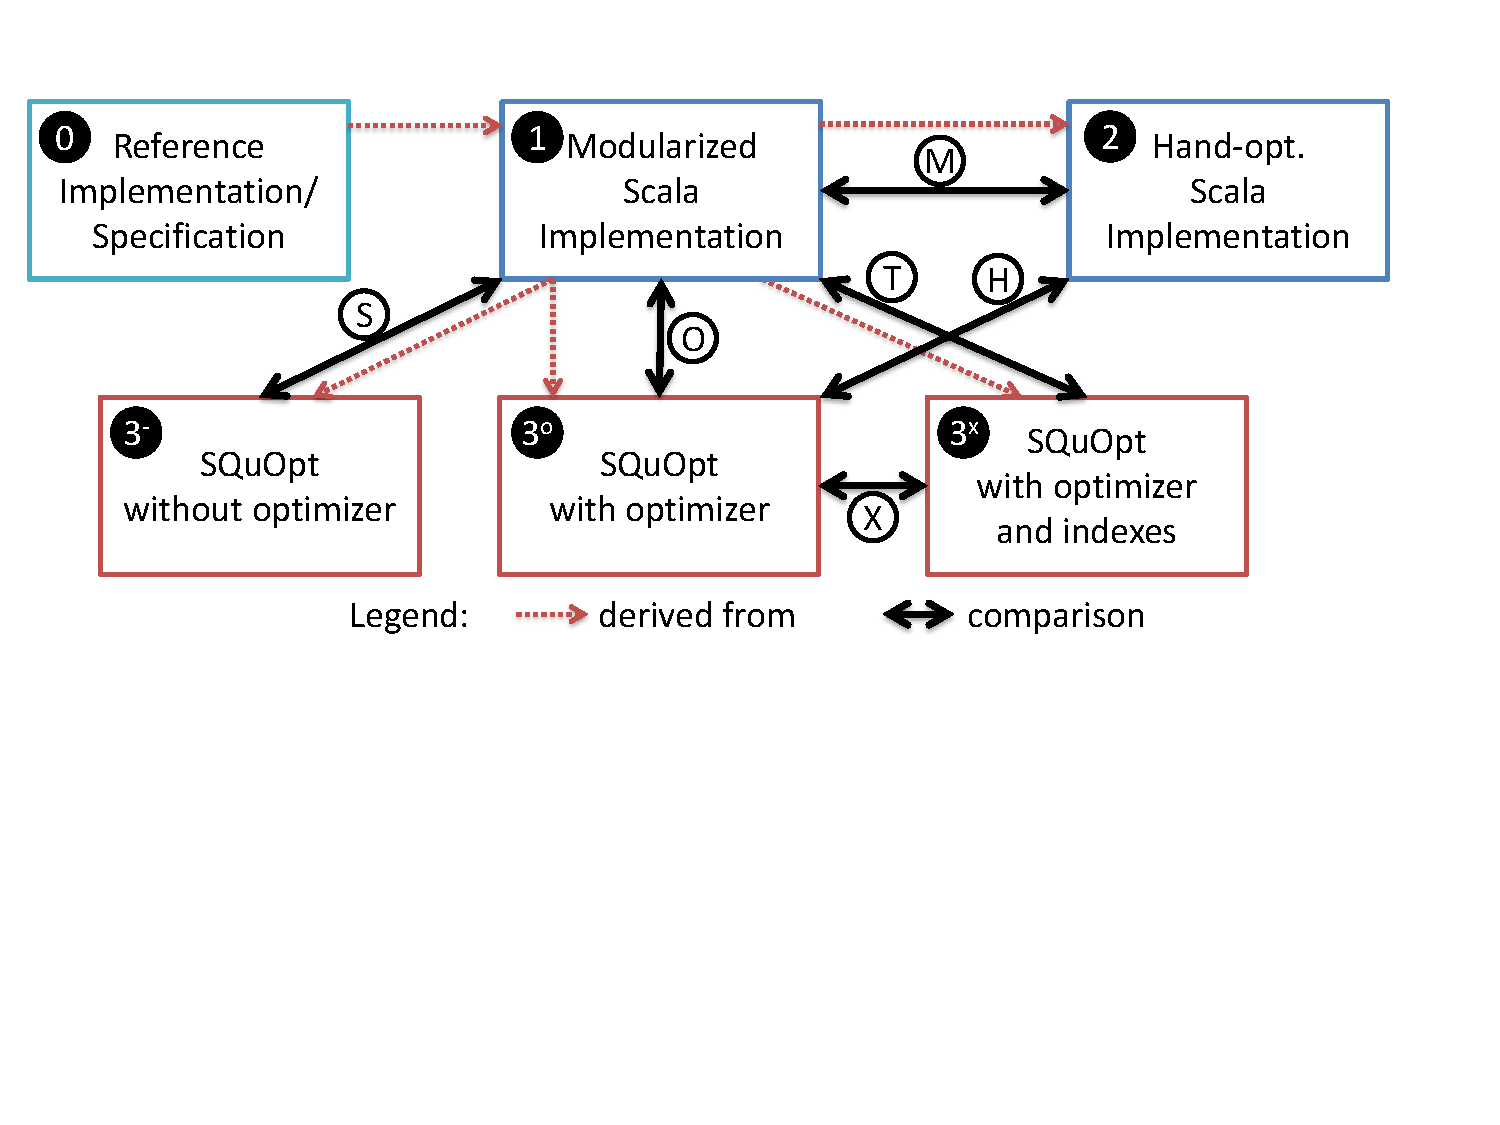
\includegraphics[width=\linewidth]{aosd13/graphs/measurements-overview}
	\caption{Measurement Setup: Overview}
	\label{fig:measurements-overview}
\end{figure}


\section{Experimental Units}




%selecting queries
%\begin{table*}
%\begin{tabular}{ll}\toprule
%Identifier & Description \\ \midrule
%PROTECTED\_FIELD % Findbugs: CI\_CONFUSED\_INHERITANCE
%%	& % Idealized: 4
%	& Class is final but declares protected field \\
%NO\_CLONE % Findbugs: CN\_IDOM
%%	& % Idealized: 9
%	&  Class implements Cloneable but does not define or use clone method \\
%SUPER\_CLONE\_MISSING % Findbugs: CN\_IDIOM\_NO\_SUPER\_CALL
%%	& % Idealized: 11
%	& The clone method does not call super.clone() \\
%NOT\_CLONEABLE % Findbugs: CN\_IMPLEMENTS\_CLONE\_BUT\_NOT\_CLONEABLE
%%	& % Idealized: 5
%	& Class defines clone() but doesn't implement Cloneable\\
%COVARIANT\_COMPARETO % Findbugs CO\_ABSTRACT\_SELF \& CO\_SELF\_NO\_OBJECT
%%	& % Idealized: 7
%	& Covariant compareTo() method defined\\
%GC\_CALL % Findbugs:  DM\_GC
%%	& % Idealized: 12
%	& Explicit garbage collection; extremely dubious except in benchmarking code\\
%RUN\_FINALIZERS\_ON\_EXIT % Findbugs DM\_RUN\_FINALIZERS\_ON\_EXIT
%%	& % Idealized: 12
%	& Method invokes dangerous method runFinalizersOnExit\\
%COVARIANT\_EQUALS %Findbugs: EQ\_ABSTRACT\_SELF
%%	& % Idealized: 4
%	& Abstract class defines covariant equals() method \\
%FINALIZER\_NOT\_PROTECTED % Findbugs: FI_PUBLIC_SHOULD_BE_PROTECTED
%%	& % Idealized: 6
%	& Finalizer should be protected, not public\\
%%NO\_SUITABLE\_CONSTRUCTOR% Findbugs: SE\_NO\_SUITABLE\_CONSTRUCTOR
%%	& % Idealized: 7
%%	& Class is Serializable but its superclass doesn't define a void constructor\\
%UNUSED\_PRIVATE\_FIELD % Findbugs: UUF\_UNUSED\_FIELD
%%	& % Idealized: 23
%	& The value of a private field is not read\\
%DONT\_CATCH\_IMSE  %Findbugs: IMSE\_DONT\_CATCH\_IMSE
%%	& % Idealized: 5
%	& Dubious catching of IllegalMonitorStateException \\\bottomrule
%\end{tabular}
%\nocaptionrule\caption{Implemented Analyses}
%\label{table:implemented-analyses}
%\end{table*}


\newcommand{\captionEvalTable}{%
As in in \cref{sec:implemenationsandspeedups}, (1) denotes the modular Scala
implementation, (2) the hand-optimized Scala one, and ($3^-$), ($3^o$), ($3^x$)
refer to the {\LoS} implementation when run, respectively, without
optimizations, with optimizations, with optimizations and indexing.
Queries marked with the $R$ superscript were selected by random sampling.}
\newcommand{\tablerowsize}{\scriptsize}
\begin{sidewaystable}[ph!]
\centering
\input{\graphPath{EvalTable}}
\nocaptionrule\caption{Performance results. \captionEvalTable}
\label{table:performance}
\end{sidewaystable}



\begin{table}[h]
  \centering
  \footnotesize
\input{\graphPath{EvalSummaryTable}}
\nocaptionrule\caption{Average performance ratios.
This table summarizes all interesting performance ratios across all queries,
using the geometric mean~\citep{Fleming86}.
The meaning of speedups is discussed in \cref{sec:implemenationsandspeedups}.}
\label{table:performanceAvg}
\end{table}

\begin{table}[h!]
\begin{tabular}{p{7cm}r}\toprule
Abstraction & Used \\ \midrule
% calculate class hierarchy & 5 \\
All fields in all class files	& 4\\
All methods in all class files	& 3\\
All method bodies in all class files	& 3\\
All instructions in all method bodies and their bytecode index	& 5\\
Sliding window (size $n$) over all instructions (and their index) &	3\\
\bottomrule
\end{tabular}\\
\nocaptionrule\caption{Description of abstractions removed during hand-optimization and number of queries where the abstraction is used (and optimized away).}
\label{table:implemented-abstractions}
\end{table}

\begin{extraEval}
\begin{table*}[tb]
\centering
\begin{tabular}{l*{3}{r@{}c@{}l}r*{2}{r@{}c@{}l}}\toprule
Name&\multicolumn{3}{c}{Base impl.\ (in ms)}&\multicolumn{3}{c}{Modular impl}&\multicolumn{3}{c}{Optimiz.\ time}&IS&\multicolumn{3}{c}{OS}&\multicolumn{3}{c}{OS-Opt}\\\midrule
\input{\graphPath{table}}
\bottomrule
\end{tabular}
\nocaptionrule\caption{Old performance results table}
\label{table:performanceOld}
\end{table*}
\end{extraEval}


As experimental units, we sampled a set of queries on code structures from FindBugs 2.0~\citep{DBLP:journals/sigplan/HovemeyerP04}. FindBugs is a popular bug-finding tool for Java Bytecode available as open source. To detect instances of bug patterns, it queries a structural in-memory representation of a code base (extracted from bytecode).
Concretely, a single loop traverses each class and invokes all visitors (implemented as listeners) on each element of the class. Many visitors, in turn, perform activities concerning multiple bug detectors which are fused together. An extreme example is that, in FindBugs, query \queryRUNFINALIZERSONEXIT{} is defined in class \code{DumbMethods} together with other 41 bug detectors for distinct types of bugs.
Typically a bug detector is furthermore scattered across the different methods of the visitor, which handle different elements of the class.
We believe this architecture has been chosen to achieve good performance; however, we do not consider such manual fusion of distinct bug detectors together as modular. We selected queries from FindBugs because they represent typical non-trivial queries on in-memory collections and because we believe our framework allows expressing them more modularly.

We sampled queries in two batches. First, we manually selected \manualQueryCount~queries (from approx.\ 400~queries in FindBugs), chosen mainly to evaluate the potential speedups of indexing (queries that primarily looked for declarations of classes, methods, or fields with specific properties, queries that inspect the type hierarchy, and queries that required analyzing methods implementation).
Subsequently, we \emph{randomly} selected a batch of \randomQueryCount~additional queries.
The batch excluded queries that rely on control-/dataflow analyses (i.e., analyzing the effect of bytecode instructions on the stack), due to limitations of the bytecode tookit we use.
In total, we have \queryCount{} queries as listed in \cref{table:performance} (the randomly selected queries are marked with the superscript $R$).




%Omit - this only showcases BAT, not our code. Show our implementation instead.
\begin{figure}[htb]
\centering
%\begin{lstlisting}
%for {
%  cf <- classFiles
%  m @ Method(_, "equals", MethodDescriptor(Seq(cf.thisClass), BooleanType), _) <- cf.methods
%  if m.isAbstract
%} yield (cf, m)
%\end{lstlisting}
%import BATLifting._
\begin{lstlisting}
for {
  classFile <- classFiles.asSquopt
  method <- classFile.methods
  if method.isAbstract && method.name ==# "equals" &&
     method.descriptor.returnType ==# BooleanType
  parameterTypes <- Let(method.descriptor.parameterTypes)
  if parameterTypes.length ==# 1 &&
     parameterTypes(0) ==# classFile.thisClass
} yield (classFile, method)
\end{lstlisting}
\caption{Find covariant \code{equals} methods.}
\label{fig:covariant-equals}
\end{figure}



%reimplementation
We implemented each query three times (see implementations (1)--(3) in \cref{sec:implemenationsandspeedups}) following the specifications given in the FindBugs documentation (0). Instead of using a hierarchy of visitors as the original implementations of the queries in FindBugs, we wrote the queries as for-comprehensions in Scala on an in-memory representation created by the Scala toolkit BAT\@.\footnote{\url{http://github.com/Delors/BAT}}
BAT in particular provides comprehensive support for
writing queries against Java bytecode in an idiomatic way.
We exemplify an analysis in \cref{fig:covariant-equals}: It detects all co-variant \code{equals} methods in a project by iterating over all class files (line 2) and all methods, searching for methods named ``\code{equals}'' that return a boolean value and define a single parameter of the type of the current class.


\smartParagraph{Abstractions}
In the reference implementations (1), we identified several reusable abstractions as shown in \cref{table:implemented-abstractions}.
The reference implementations of all queries except \querySEBADFIELDINNERCLASS{} use exactly one of these abstractions, which encapsulate the main loops of the queries.

\smartParagraph{Indexes}
For executing ($3^x$) (\LoS\ with indexes), we have constructed three indexes to speed up navigation over the queried data of queries 1--\manualQueryCount{}: Indexes for method name, exception handlers, and instruction types. We illustrate the implementation of the method-name index in \cref{fig:indexes}: it produces a collection of all methods and then indexes them using \code{indexBy}; its argument extracts from an entry the key, that is the method name.
We selected which indexes to implement using guidance from \LoS{} itself; during optimizations, \LoS{} reports which indexes it could have applied to the given query. Among those, we tried to select indexes giving a reasonable compromise between construction cost and optimization speedup.
%% If we want to show the raw data, we could use this LaTeX code - but we need updated, and correct, data!
We first measured the construction cost of these indexes:

\begin{center}
\begin{tabular}{l*{1}{r@{}c@{}l}}\toprule
Index&\multicolumn{3}{c}{Elapsed time (ms)}\\\midrule

Method name&$97.99$&$\pm$&$2.94$\\
Exception handlers&$179.29$&$\pm$&$3.21$\\
Instruction type&$4166.49$&$\pm$&$202.85$\\

\bottomrule
\end{tabular}
\end{center}
For our test data, index construction takes less than 200 ms for the first two indexes, which is moderate compared to the time for loading the bytecode in the BAT representation ($\readingClassFilesTime$). Building the instruction index took around 4 seconds, which we consider acceptable since this index maps each type of instruction (e.g.\ \code{INSTANCEOF}) to a collection of all bytecode instructions of that type.
%Valid question: why does the exception-handler index take so much more than the query it optimizes? That's because indexes are interpreted. But it's best not to say it. Also, we already discuss this later convincingly.

%The first index maps any method name to the corresponding methods (together with containing classes), and is used by many different queries. Its implementation is shown in \cref{fig:indexes}: the code shown first produces a collection of all methods and then indexes them using \code{indexBy}; its argument extracts from an entry the key, that is the method name.
%The second index maps any exception type to exception handlers catching them (together with the containing method bodies, methods and class).
%The third index allows to look for occurrences of bytecode instructions of a given type; it maps any type of bytecode instruction (like \code{INVOKESTATIC}, \code{INVOKEVIRTUAL} and so on) to its occurrences.

\begin{figure}
\centering
\begin{lstlisting}
val methodNameIdx: Exp[Map[String, Seq[(ClassFile, Method)]]] = (for {
  classFile <- classFiles.asSquopt
  method <- classFile.methods
} yield (classFile, method)).indexBy(entry => entry._2.name)
\end{lstlisting}
\caption{A simple index definition}
\label{fig:indexes}
\end{figure}



\section{Measurement Setup}
To measure performance, we executed the queries on the preinstalled JDK class library (\texttt{rt.jar}), containing 58M of uncompressed Java bytecode.
We also performed a preliminary evaluation by running queries on the much smaller ScalaTest library, getting comparable results that we hence do not discuss.
Experiments were run on a 8-core Intel Core i7-2600, 3.40 GHz, with 8 GB of RAM, running Scientific Linux release 6.2.
The benchmark code itself is single-threaded, so it uses only one core; however the JVM used also other cores to offload garbage collection.
We used the preinstalled OpenJDK Java version 1.7.0\_05-icedtea and Scala 2.10.0-M7.

We measure steady-state performance as recommended by \citet{Georges07rigorousJavaPerformance}. We invoke the JVM $p = 15$ times;
at the beginning of each JVM invocation, all the bytecode to analyze is loaded in memory and converted into BAT's representation.
In each JVM invocation, we iterate each benchmark until the variations of results becomes low enough. We measure the variations of results through the coefficient of variation (CoV; standard deviation divided by the mean). Thus, we iterate each benchmark until the CoV in the last $k = \kZrememberedSampleLoops$ iterations drops under the threshold $\theta = \thetaZmaxCov$, or until we complete $q = \qZmaxLoops$ iterations.
We report the arithmetic mean of these measurements (and also report the usually low standard deviation on our web page).
%PG: I had p = 3, k = 50, theta = 0.02, q = 1000, but changed the parameters when running more queries.

\section{Results}

\smartParagraph{Correctness} We machine-checked that for each query, all variants in \cref{table:performance} agree.

\smartParagraph{Modularization Overhead}
We first observe that performance suffers significantly when using the abstractions we described in \cref{table:implemented-abstractions}. These abstractions, while natural in the domain and in the setting of a declarative language, are not idiomatic in Java or Scala because, without optimization, they
will obviously lead to bad performance. They are still useful abstractions from the point of view of modularity, though---as indicated by \cref{table:implemented-abstractions}---and as such it would be desirable if one could use them without paying the performance penalty.


\smartParagraph{Scala Implementations vs.\ FindBugs}
Before actually comparing between the different Scala and \LoS\ implementations, we first ensured that the implementations are comparable to the original FindBugs implementation. A direct comparison between the FindBugs reference implementation and any of our implementations is not possible in a rigorous and fair manner. FindBugs bug detectors are not fully modularized, therefore we cannot reasonably isolate the implementation of the selected queries from support code. Furthermore, the architecture of the implementation has many differences that affect performance: among others, FindBugs also uses multithreading. Moreover, while in our case each query loops over all classes, in FindBugs, as discussed above, a single loop considers each class and invokes all visitors (implemented as listeners) on it.

We measured \emph{startup performance}~\citep{Georges07rigorousJavaPerformance}, that is the performance of running the queries only once, to minimize the effect of compiler optimizations.
We setup our \LoS-based analyses to only perform optimization and run the optimized query. To setup FindBugs, we manually disabled all unrelated bug detectors; we also made the modified FindBugs source code available. The result is that the performance of the Scala implementations of the queries ($3^-$) has performance of the same order of magnitude as the original FindBugs queries -- in our tests, the \LoS\ implementation was about twice as fast. However, since the comparison cannot be made fair, we refrained from a more detailed investigation.

% XXX HACK
\smartParagraph{SQuOpt Overhead and Optimization Potential}
We present the results of our benchmarks in \cref{table:performance}.
Column names refer to a few of the definitions described above; for readability, we do not present all the ratios previously introduced for each query, but report the raw data.
In \cref{table:performanceAvg}, we report the geometric mean \cite{Fleming86} of each ratio, computed with the same weight for each query.

%queries are between \maxInterpOver{}x slower and \maxInvInterpOver{}x faster; on average \LoS\ queries are \geoMeanInvInterpOver{}x faster.
%\minInvInterpOver{}x and \maxInvInterpOver{}x---that is, queries are between \minInterpOver{}x and
We see that, in its current implementation, \LoS\ can cause a overhead S
(1/$3^-$) up to \maxInterpOver{}x. On average \LoS\ queries are
\geoMeanInterpOver{}x faster. These differences are due to minor implementation
details of certain collection operators.
For query $18^R$, instead, we have that the the basic \LoS\ implementation is \maxInvInterpOver{}x faster and are investigating the reason; we suspect this might be related to the use of pattern matching in the original query.

As expected, not all queries benefit from optimizations;
out of \queryCount{} queries, optimization affords for \nSpeededUpQueries{} of them significant speedups ranging from a \minOptimSpeedup{} factor to a \maxOptimSpeedup{} factor; \nBigSpeededUpQueries{} queries are faster by a factor of at least \speedupBigThreshold{}.
Only queries \queryMSPKGPROTECT{}, \querySICINNERSHOULDBESTATICANON{} and \queryITAINEFFICIENTTOARRAY{} fail to recover any modularization overhead.

We have analyzed the behavior of a few queries after optimization, to understand why their performance has
(or has not) improved.

Optimization makes query \querySEBADFIELDINNERCLASS{} slower; we believe this is because optimization replaces filtering by lazy filtering, which is usually faster, but not here.
Among queries where indexing succeeds, query \queryGCCALL{} has the least speedup. After optimization, this query uses the instruction-type index to find all occurrences of invocation opcodes (\code{INVOKESTATIC} and \code{INVOKEVIRTUAL}); after this step the query looks, among those invocations, for ones targeting \code{runFinalizersOnExit}. Since invocation opcodes are quite frequent, the used index is not very specific, hence it allows for little speedup (\speedupTGCCALL). However no other index applies to this query; moreover, our framework does not maintain any selectivity statistics on indexes to predict these effects.
Query \queryFIUSELESS{} benefits from indexing without any specific tuning on our part, because it looks for implementations of \code{finalize} with some characteristic, hence the highly selective method-name index applies.
After optimization, query \queryDONTCATCHIMSE{} becomes simply an index lookup on the index for exception handlers, looking for handlers of \code{IllegalMonitorStateException}; it is thus not surprising that its speedup is thus extremely high (\maxOptimSpeedup{}). This speedup relies on an index which is specific for this kind of query, and building this index is slower than executing the unoptimized query. On the other hand, building this index is entirely appropriate in a situation where similar queries are common enough. Similar considerations apply to usage of indexing in general, similarly to what happens in databases.

\smartParagraph{Optimization Overhead}
The current implementation of the optimizer is not yet optimized for speed (of the optimization algorithm). For instance, expression trees are traversed and rebuilt completely once for each transformation.
However, the optimization overhead is usually not excessive and
is $\avgOptimTime \pm \stdDevOptimTime$ ms, varying between \minOptimTime{} ms and \maxOptimTime{} ms (mostly depending on the query size).

\smartParagraph{Limitations}
Although many speedups are encouraging, our optimizer is currently a proof-of-concept and we experienced some limitations:
\begin{itemize}
\item In a few cases hand-optimized queries are still faster than what the optimizer can produce. We believe these problems could be addressed by adding further optimizations.
\item Our implementation of indexing is currently limited to immutable collections. For mutable collections, indexes must be maintained incrementally.
Since indexes are defined as special queries in {\LoS},  incremental index maintenance becomes an instance of incremental maintenance of query results, that is, of incremental view maintenance. We plan to support incremental view maintenance as part of future work; however,
indexing in the current form is already useful, as illustrated by our experimental results.
\end{itemize}

\smartParagraph{Threats to Validity}
With rigorous performance measurements and the chosen setup, our study was setup to maximize internal and construct validity. Although we did not involve an external domain expert and we did not compare the results of our queries with the ones from FindBugs (except while developing the queries), we believe that the queries adequately represent the modularity and performance characteristics of FindBugs and {\LoS}. However, since we selected only queries from a single project, external validity is limited.
While we cannot generalize our results beyond FindBugs yet, we believe that the FindBugs queries are representative for complex in-memory queries performed by applications.


\smartParagraph{Summary}
We demonstrated on our real-world queries that relying on declarative abstractions in collection queries often causes a significant slowdown. As we have seen, using \LoS\ without optimization, or when no optimizations are possible, usually provides performance comparable to using standard Scala; however, \LoS\ optimizations can in most cases remove the slowdown due to declarative abstractions. Furthermore, relying on indexing allows to achieve even greater speedups while still using a declarative programming style.
Some implementation limitations restrict the effectiveness of our optimizer, but since this is a preliminary implementation, we believe our evaluation shows the great potential of optimizing queries to in-memory collections.


% vim: set tw=0:


\section{Related Work}
\label{sec:relwork}
This paper builds on prior work on language-integrated queries, query optimization, techniques for DSL embedding, and other works on code querying.

\smartParagraph{Language-Integrated Queries}
Microsoft's Language-Integrated Query technology (\LINQ)~\citep{Meijer:2006:LRO:1142473.1142552,Bierman:2007:LTF:1297027.1297063} is similar to our work in that it also
reifies queries on collections to enable analysis and optimization. Such queries can be executed against a variety of backends (such as SQL databases or in-memory objects), and adding new back-ends is supported. Its implementation uses \emph{expression trees}, a compiler-supported
implicit conversion between expressions and their reification as a syntax tree. There are various major differences, though.
First, the support for expression trees is hard-coded into the compiler. This means that the techniques are not applicable in languages 
that do not explicitly support expression trees. More importantly, the way expression trees are created in \LINQ\ is generic and fixed.
For instance, it is not possible to create different tree nodes for method calls that are relevant to an analysis (such as the \code{map} method) than for method calls that are irrelevant for the analysis (such as the \code{toString} method). For this reason, expression trees in \LINQ\ 
cannot be customized to the task at hand and contain too much low-level information. It is well-known that this makes it quite hard to
implement programs operating on expression trees~\citep{Eini11Pain}. 

\LINQ\ queries can also not easily be decomposed and modularized. For instance, consider the task of refactoring the filter in the query {\tt from x in y where x.z == 1 select x}
into a function. Defining this function as {\tt bool comp(int v) \{ return v == 1; \}} would destroy the possibility of analyzing the filter for optimization, since
the resulting expression tree would only contain a reference to an opaque function. The function could be declared as returning an expression tree instead, but then
this function could not be used in the original query anymore, since the compiler expects an expression of type {\tt bool} and not an expression tree of type {\tt bool}.
It could only be integrated if the expression tree of the original query is created by hand, without using the built-in support for expression trees.

% Klaus: since we do not talk much about the embedding technique we should not talk about type safety here
%Expression trees in \LINQ\ also provide little type safety. While they appear to be typed superficially (quoting an expression of type \code{T} yields 
%an expression tree of type \code{Expression<T>}) they are untyped internally. For instance, when one decomposes a node into its components,
%the components are untyped. 
% Klaus: let's not distract by talking superficially about Haskell
% This is similar to deep embedding of expressions in Haskell, which typically use a phantom type wrapper around untyped expressions.

%In contrast, expression trees in our approach are typed and simple transformations can be statically checked to be type-preserving. More complex optimizations require however type casts and rely on erasure of type parameters at run time, as we will discuss in detail later on.

Although queries against in-memory collections could theoretically also be optimized in \LINQ, the standard implementation, {\LINQ}2Objects, performs no optimizations. 

A few optimized embedded DSLs allow executing queries or computations on distributed clusters.
DryadLINQ~\citep{Yu08}, based on \LINQ, optimizes queries for distributed
execution. It inherits \LINQ's limitations and thus does not support decomposing queries in different modules.
Modularizing queries is supported instead by FlumeJava~\citep{Chambers10},
another library (in Java) for distributed query execution.
However, FlumeJava cannot express many optimizations because its representation
of expressions is more
limited; also, its query language is more cumbersome. Both problems are rooted
in Java's limited support for embedded DSLs.
Other embedded DSLs support parallel platforms such as GPUs or many-core CPUs,
such as Delite~\citep{Rompf13}.

\citet{Willis06JQL,Willis08} add first-class queries to Java through a source-to-source translator and implement a few selected optimizations, including join order optimization and incremental maintenance of query results.
They investigate how well their techniques apply to Java programs, and they suggest that programmers use manual optimizations to avoid expensive constructs like nested loops. While the goal of these works is similar to ours, their implementation as an external source-to-source-translator makes
the adoption, extensibility, and composability of their technique difficult%
%~\citep{ErdwegGR12}
.
%KO: not sure whether the reference here helps
%PG: Remove it if we have space limits.

There have been many approaches for a closer integration of SQL queries into programs, such as
HaskellDB~\citep{Leijen99DSEC} (which also inspired \LINQ), or Ferry~\citep{Grust:2009:FDP:1559845.1559982} 
(which moves part of a program execution to a database). In Scala, there are also
APIs which integrate SQL queries more closely such as
Slick.\footnote{\url{http://slick.typesafe.com/}} Its frontend allows to define
and combine type-safe queries, similarly to ours (also in the way it is
implemented).
However, the language for defining queries maps to SQL, so it does not support nesting collections
in other collections (a feature which simplified our example in
Sec.~\ref{sec:motivation}), nor distinguishes statically between different kinds of
collections, such as \code{Set} or \code{Seq}.
Based on Ferry, ScalaQL~\citep{JOT:issue_2010_07/article3} extends Scala with a compiler-plugin to integrate a query language on top of a relational database. The work by \citet{Spiewak09scalaql:language-integrated} is
 unrelated to~\citep{JOT:issue_2010_07/article3} but also called ScalaQL\@. It is similar to our approach in that it also 
proposes to reify queries based on for-comprehensions, but it is not clear from the paper how the reification 
works.\footnote{We contacted the authors; they were not willing to provide more details or the sources of their approach.}


\smartParagraph{Query Optimization}
Query optimization on relational data is a long-standing issue in the database community, but there
are also many works on query optimization on objects~\citep{Fegaras00,Grust99PhD}.
Compared to these works, we have only implemented a few simple query optimizations, so there is potential
for further improvement of our work by incorporating more advanced optimizations.

%CQEngine (\url{http://code.google.com/p/cqengine/}) does not support path
%indexes. It support standing queries - but those are just incrementally
%maintained queries, as far as it seems. But the system is quite cool.
%---

% That's not strictly true, and is not the point. The point is a consequence: in a monoid comprehension for a given monoid, a generator cannot range over a monoid which is weaker wrt.\ idempotence or commutativity.

%For instance, while the formal analogous of folds in their calculus is a monoid homomorphism, computing the size of a Set can be expressed through a fold but not through a monoid homomorphism, since it is a fold from an idempotent to a non-idempotent monoid.

% Klaus: I think this is not that relevant for ICSE
%\citet{Henglein10} present an embedding of the relational algebra in Haskell.
%Queries are not reified in their approach, but due to a particularly sophisticated
%representation of multisets it is possible to execute some queries containing
%cross-products using faster equi-joins.


\smartParagraph{Scala and DSL Embedding}
\label{sec:rwdsl}
Technically, our implementation of \LoS\ is a deep embedding of a part of the Scala collections API~\citep{odersky2009fighting}.
Deep embeddings were pionereed by \citet{Leijen99DSEC} and \citet{elliott03compiling}. The technical
details of the embedding are not the main topic of this paper; we are using some of the 
Scala techniques presented by \citet{rompf2010lightweight} for using implicits and for
adding infix operators to a type. Similar to \citet{rompf2010lightweight}, we also 
use the Scala compiler on-the-fly. A plausible alternative backend for \LoS\ would
have been to use Delite~\citep{Rompf11BBlocks}, a framework for
building highly efficient DSLs in Scala.
Using this framework, in concurrent work, \citet{Rompf13} also optimize
collection queries; while their work allows for imperative programs, they do
not support embedding arbitrary libraries in an automated way. On the other
hand, they can reuse support for automatic parallelization and multiple platforms present in Delite.
\citet{Ackermann12} present Jet, which also optimizes collection queries but
targets MapReduce-style computations in a distributed environment.
Moreover, both works do not apply typical database optimizations such as
indexing or filter hoisting.


We regard the Scala collections API~\citep{odersky2009fighting} as a shallowly embedded query DSL\@. Query operators immediately perform collection operations when called, so that it is not possible to optimize queries before execution. In addition to these eager query operators, the Scala collections API also provides \emph{views} to create lazy collections.
Views are somewhat similar to {\LoS} in that they reify query operators as data structures and interpret them later.
However, views are not used for automatic query optimization, but for explicitly changing the evaluation order of collection processing. Unfortunately, views are not suited as a basis for the implementation of {\LoS} because they only reify the outermost pipeline of collection operators, whereas nested collection operators as well as other Scala code in queries, such as filter predicates or \code{map} and \code{flatMap} arguments, are only shallowly embedded.
Deep embedding of the whole query is necessary for many optimizations, as discussed in Sec.~\ref{sec:solution}.

\smartParagraph{Code Querying}
In our evaluation we explore the usage of \LoS\ to express queries on code and re-implement a subset of the FindBugs~\citep{DBLP:journals/sigplan/HovemeyerP04} analyses. There are various other specialized code query languages such as 
CodeQuest~\citep{Hajiyev06CodeQuest} or D-CUBED~\citep{Wegrzynowicz:2009:GBU:1639950.1640032}. 
Since these are special-purpose query languages that are not embedded into a host language, they are not directly comparable to our approach.



\section{Future Work}
As part of future work we plan to add support for \emph{incremental view
maintenance}~\citep{GlucheGrust97Incr} to \LoS. This would allow, for instance,
to update incrementally both indexes and query results.

To make our DSL more convenient to use, it would be useful to use the
virtualized pattern matcher of Scala 2.10, when it will be more robust, to add
support for pattern matching in our virtualized queries.

Finally, while our optimizations are type-safe, as they rewrite an expression
tree to another of the same type, currently the Scala
type-checker cannot verify this statically, because of its limited support for
GADTs.
Solving this problem conveniently would allow checking statically that
transformations are safe and make developing them easier.

\section{Conclusions}
\label{sec:concl}

We have illustrated the tradeoff between performance and modularity for queries on in-memory collections. We have shown that it is possible to design a deep embedding of a version of the collections API which reifies queries and can optimize them at runtime.
Writing queries using this framework is, except minor syntactic details, the same as writing queries using the collection library, hence the adoption barrier to using our optimizer is low. 

Our evaluation shows that using abstractions in queries introduces a significant
performance overhead with native Scala code, while \LoS{}, in most cases, makes
the overhead much more tolerable or removes it completely. Optimizations are not
sufficient on some queries, but since our optimizer is a proof-of-concept with
many opportunities for improvement, we believe a more elaborate version will
achieve even better performance and reduce these limitations.


%\section*{Acknowledgements}
\smartParagraph{Acknowledgements}
The authors thank Sebastian Erdweg for helpful discussions on
this project, Katharina Haselhorst for help
implementing the code generator, and the anonymous reviewers, Jacques Carette and Karl Klose
for their helpful comments on this paper.
This work is supported in part by the European Research Council, grant \#203099 ``ScalPL''.
